%!TEX TS-program = xelatex
%!TEX encoding = UTF-8 Unicode

\documentclass[12pt]{extarticle}
% extarticle is like article but can handle 8pt, 9pt, 10pt, 11pt, 12pt, 14pt, 17pt, and 20pt text

\def \ititle {Philosophical Psychology}

\def \isubtitle {Lecture 07}

\def \iauthor {Stephen A. Butterfill}
\def \iemail{s.butterfill@warwick.ac.uk}
\date{}

%for strikethrough
\usepackage[normalem]{ulem}

\input{$HOME/latex_imports/preamble_steve_handout}

%\bibpunct{}{}{,}{s}{}{,}  %use superscript TICS style bib
%remove hanging indent for TICS style bib
%TODO doesnt work
\setlength{\bibhang}{0em}
%\setlength{\bibsep}{0.5em}


%itemize bullet should be dash
\renewcommand{\labelitemi}{$-$}

\begin{document}

\begin{multicols*}{3}

\setlength\footnotesep{1em}


\bibliographystyle{newapa} %apalike

%\maketitle
%\tableofcontents




%---------------
%--- start paste


\def \ititle {07: Three Questions about Mindreading}

\begin{center}

{\Large

\textbf{\ititle}

}



\iemail %

\end{center}



\section{Nonhuman Mindreading}


Many animals including scrub jays \citep{Clayton:2007fh},
ravens \citep{bugnyar:2016_ravens},
goats \citep{kaminski:2006_goats},
dogs \citep{kaminski:2009_domestic},
ringtailed lemurs \citep{sandel:2011_evidence},
monkeys \citep{burkart:2007_understanding, hattori:2009_tufted}
and chimpanzees \citep{melis:2006_chimpanzees,karg:2015_chimpanzees,krupenye:2016_great} reliably vary their actions in ways that are appropriate given facts about another’s mental states.
What could underpin such abilities to track others’ mental states?

Example 1: ‘In informed trials dominant individuals witnessed the experimenter hiding
food behind one of the occluders whereas in uninformed trials they could
not see the baiting procedure. In misinformed trials, dominants witnessed
the experimenter hiding food behind one of the occluders, and once the
dominant’s visual access was blocked, the experimenter switched the food
from its original location to the other occluder’ \citep{Hare:2001ph}.

Example 2: ‘the jays were much more likely to re-cache if they had been observed by a conspecific while they
were caching than when they had cached in private. By re-caching items that the observer had seen
them cache, the cachers significantly reduce the chance of cache theft, as observers would be unable
to rely on memory to facilitate accurate cache theft’ \citep[p.~516]{Clayton:2007fh}.

Example 3: ‘ravens can transfer knowledge from their own experience in a novel context---using peepholes to look
into an adjacent room---to a caching situation in which they can hear but not see a conspecific in that
room’ \citep{bugnyar:2016_ravens}.

\section{Question 1: Tracking to Representing}

How do observations about tracking support conclusions about representing?

‘Comparative psychologists test for \emph{mindreading} in non-human animals by determining whether they
\emph{detect} the presence and absence of particular cognitive states in a wide variety of
circumstances.
They eliminate potential confounding variables by ensuring that there is no one
observable state to which subjects might be responding’
\citep[p.~487]{halina:2015_there}.

For you to \emph{track} someone’s mental state (such as a belief that there is food behind that rock)
is for there to be a process in you which nonaccidentally depends in some way on whether she has that
mental state.



‘chimpanzees understand … intentions … perception and knowledge,’ but ‘chimpanzees probably do not
understand others in terms of a fully human-like belief–desire psychology’
\citet[p.~191]{Call:2008di}.

‘the core theoretical problem in contemporary research on animal mindreading is that the bar—the
conception of mindreading that dominates the field—is too low, or more specifically, that it is
too underspecified to allow effective communication among researchers, and reliable
identification of evolutionary precursors of human mindreading through observation and experiment’
\citep[p.~318]{heyes:2014_animal}

 
\section{Question 2: Dissociations}

Why are there  dissociations in nonhuman apes’, human infants’ and human adults’ performance on belief-tracking tasks?

\begin{center}

  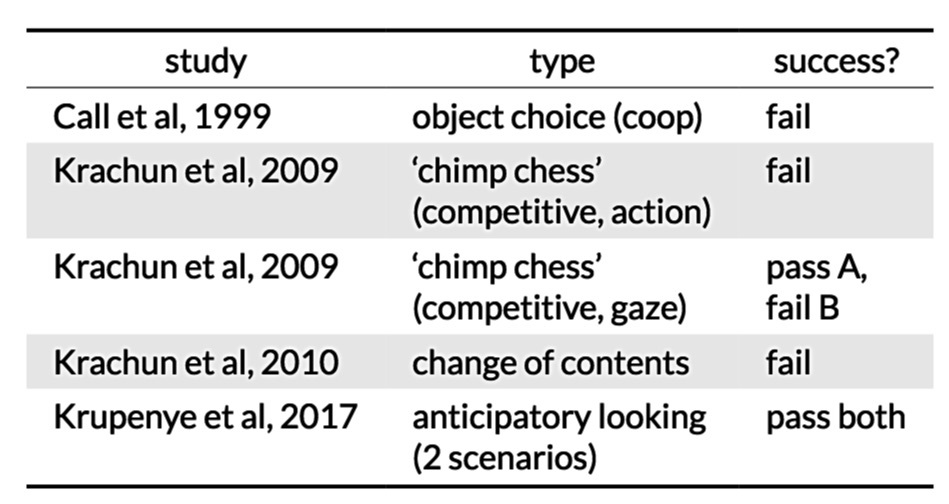
\includegraphics[width=0.30\textwidth]{fig/dissociation_table.jpg}
  
  \end{center}
  
‘the present evidence may constitute an implicit understanding of belief’
\citep[p.~113]{krupenye:2016_great}



 
\section{Question 3: Automaticity}

Are human adults’ abilities to track others’ beliefs automatic?

For our purposes, a process is \emph{automatic} to the degree that whether it occurs is independent of
its relevance to the particulars of the subject's task, motives and aims.  \emph{automatic mindreading} is mindreading that is a consequence of
automatic processes only.


There is evidence that some mindreading in human adults is
 automatic
\citep[e.g.][]{kovacs_social_2010,Schneider:2011fk,Wel:2013uq} and
that not all mindreading in human adults is
\citep{apperly:2008_back,apperly_why_2010,Wel:2013uq}.

‘Participants never reported belief tracking when questioned in an open format after the experiment
(“What do you think this experiment was about?”). Furthermore, this verbal debriefing about the
experiment’s purpose never triggered participants to indicate that they followed the actor’s belief
state’ \citep[p.~2]{Schneider:2011fk}.
(Note that there are relevant failures to replicated this paradigm.)


For adults (and children who can do this),
representing perceptions and beliefs as such---and even merely holding in mind
what another believes, where no inference is required---involves a measurable
processing cost \citep{apperly:2008_back,apperly:2010_limits}, consumes attention
and working memory in fully competent adults \citealp{Apperly:2009cc,
lin:2010_reflexively, McKinnon:2007rr},  may require inhibition \citep{bull:2008_role}
and makes demands on executive function \citep{apperly:2004_frontal,samson:2005_seeing}.

\textbf{Q3b: How could
belief-tracking ever be automatic if it significantly depends on working memory and consumes attention?}


%--- end paste
%---------------

\footnotesize
\bibliography{$HOME/endnote/phd_biblio}

\end{multicols*}

\end{document}
